\Def Назовём \textit{предельной точкой языка $\F$} такое $\alpha$, что в любой окрестности $\alpha$ существует $\alpha'$, для которого не выполнен закон нуля или единицы для языка $\F$.

Иначе говоря, множество предельных точек языка~--- это множество предельных точек объединения спектров всех его формул.

Докажем, что в языке $\mathcal{L}^3$ предельные точки существуют в любой левой полуокрестности единицы: 
$\forall \varepsilon > 0 ~ \exists \alpha \in (1 - \varepsilon, 1)$, $\alpha$~---предельная точка.

Рассмотрим граф, состоящий из $k+2$ треугольников, соединённых простыми путями.
Причём, расстояние (в рёбрах) между вторым и третьим треугольниками, третьим и четвёртым и т. д., одинаково.
Обозначим это расстояние $m$, а расстояние между первым и вторым треугольником~--- $s$.

\begin{figure}[h]
    \centering
  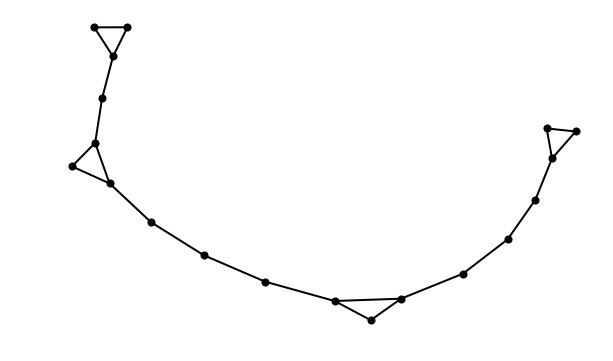
\includegraphics[scale=0.4]{picrel/Hksm.png}
  \caption{Граф с $k = 2$, $s = 2$ и $m = 4$}
  \label{fig:chain1}
\end{figure}

Плотность такого графа равна 
$$\rho({H_{ksm}}) = \dfrac{6+s + (3+m)k}{5+s + (2+m)k}$$
и при увеличении $k$ стремится к $\rho_\infty = \dfrac{3+m}{2+m}$.

Граф с $k=0$ состоит из двух треугольников и имеет вид гантели.

Т.к. 
$sign\left(\dfrac{\partial\rho({H_{ksm}})}{\partial k}\right) = sign(3+s-m)$,
то при $m < 3 + s$ плотность графа растёт при увеличении  $k$ и, как нетрудно убедиться, при этом выполнено равенство
$\rho({H_{ksm}}) = \rho^{max}({H_{ksm}})$.
Будем считать $m = s+2$, т.к. при таком соотношении длины гантели и длины добавочных звеньев
граф получается оптимальным с точки зрения плотности, что пригодится в дальнейшем.

Таким образом, по теореме \ref{th:bollobash}, для доказательства утверждения достаточно предъявить для каждого такого графа формулу из  $\mathcal{L}^3$, выражающую его существование.

% Для удобства дальнейших рассуждениях введём следующее понятие.
% Пусть имеется граф $G$.

% \Def \textit{Подстановкой} называется отображение, которое ставит в соответствие каждой переменной формулы в зоне действия квантора по этой переменной некоторую вершину графа $G$.

% При фиксированной подстановке одной переменной в зонах действия разных кванторов по этой переменной  могут соответствовать разные вершины.

Вместо 
$\exists x \exists y \exists z ~ x \sim y \wedge y \sim z \wedge x \sim z$
будем писать 
$\triangle_{xyz}$

Рассмотрим формулу
\[ \varphi_{0s} = \triangle_{xyz} \wedge \psi_s^{x},\]
\begin{equation}
\label{f:gantel}
\begin{split}
\psi_s^x &= \exists x ~ 
    \left[ x \sim z \wedge x \neq y \wedge x \nsim y  \right] \\
&\wedge \exists y ~
    \left[ y \sim x \wedge y \neq z \wedge y \nsim z \right] \\
&\wedge \exists z ~
    \left[ z \sim y \wedge z \neq x \wedge z \nsim x  \right] \\
&\wedge ~ \qquad \qquad \cdots \\
&\wedge \exists \xi ~ 
    \xi \sim \nu \wedge \xi \sim \eta,
\end{split}
\end{equation}
где количество выражений в квадратных скобках в $\psi_{s}^{x}$ равно $s+1$; верхний индекс $x$ соответствует переменной, стоящей после первого квантора существования, вместо символа $\xi$ стоит одна из переменных $x,y,z$~--- какая именно, определяется параметром $s$ (переменные у кванторов существования следуют в циклическом порядке: $x,y,z,x,y, \ldots$); $\nu$ и $\eta$~--- две оставшиеся из $x,y,z$ переменные, отличные от $\xi$. 

Если бы в этой формуле после каждого нового квантора существования присутствовало условие на то, что переменная, стоящая после квантора не равна всем переменным, объявленным ранее, то $\varphi_{0s}$ выражала бы существование гантели c расстоянием между треугольниками, равным $s$ (это не совсем так, потому что наша формула запрещает проведение некоторых рёбер, соединяющих вершины гантели, но это ничего не портит ни для гантели, ни для $H_{ksm}$:  при $\alpha = 1/\rho(H_{ksm})$ графов $H_{ksm}$ c дополнительными рёбрами а.п.н. нет в $\Gna$). 
К сожалению, имея лишь три переменных, мы не можем напрямую запретить одной переменной соответствовать нескольким вершинам, поэтому $G \vDash \varphi_{0s}$ не только в случае, когда граф $G$ содержит гантель соответствующей длины (например, граф, изображённый на на Рис. \ref{fig:reuse intermediate}, удовлетворяет $\varphi_{0,6}$).
Впрочем, как мы покажем далее, делать это и не обязательно.

Составим теперь аналогичную формулу $\varphi_{ksm}$ для графа $H_{ksm}$:

\[ \varphi_{ksm} =  \triangle_{xyz} \wedge \psi_{s}^{x} \wedge \psi_{m}^{\xi_1} \wedge \ldots \wedge \psi_{m}^{\xi_{k}} .\]
Здесь $\xi_1$~--- следующая по порядку ($x,y,z,x,y,\ldots$) переменная после переменной, стоящей у последнего квантора существования в $\psi^x_s$, $\xi_2$~--- следующая после переменной, стоящей у последнего квантора существования в $\psi^{\xi_1}_s$ и т. д.

%\underbrace{\psi_{m}^{\xi_1} \wedge \ldots \wedge \psi_{m}^{\xi_{k}}}_{\text{k раз}}

% \begin{equation}
% \label{f:phiKsm}
% \left. 
%     \begin{split}
%         \exists x~\triangle_{xyz} 
%         \gantelRightPart
% \right\}
% \left. 
%     \left. \gantelRightPart \right\}
%     \left. \gantelRightPart \right\}
% \right\}
% \end{equation}

% \[
% \begin{split}
% \left.
% a = b \\
% c = d
% \right\}
% \end{split}
% \]

По той же причине, существование в $\Gna$ подграфа $H_{ksm}$ не является необходимым для того, чтобы формула $\varphi_{ksm}$ была верна.
Однако, оно становится необходимым (c вероятностью, стремящейся к единице) при $\alpha = 1/\rho_{H_{ksm}}$ и $m = s+2$. 
Действительно, докажем следующую лемму.

\begin{Lem} 
\label{lem:min_ro_Hksm}
% Граф $H_{ksm}$ имеет минимальную $\rho^{max}$ среди всех графов, для которых выполнено $\varphi_{ksm}$.
Пусть $k \in \{0\} \cup \N,~s \in \N,~ m=s+2$. Если $G \vDash \varphi_{ksm}$, и $G$ не содержит подграфа, изоморфного $H_{ksm}$, то $G$ содержит более плотный подграф с меньшим числом вершин.
\end{Lem}

\begin{proof}
Назовём \textit{переменной*} переменную в зоне действия квантора по этой переменной.
Так, одной букве-переменной $x$ соответствует несколько переменных со звёздочкой.

В графе $H_{ksm}$ каждой переменной* формулы $\varphi_{ksm}$ соответствует отдельная вершина.
Пусть для графа $G$ истинна $\varphi_{ksm}$, и он не содержит подграфа, изоморфного $H_{ksm}$.
% то он имеет вершину, которой соответствует более одной переменной.
% Далее будем рассматривать только второй случай.
% Пусть в звене под номером $k'$ (номер $0$ соответствует гантели), впервые произошло повторное ``использование'' вершины. 

$G \vDash \varphi_{ksm}$
означает, что существует (по крайней мере, одно) такое отображение из множества переменных* формулы во множество вершин графа, что если в формулу вместо переменных подставить соответствующие вершины и убрать кванторы, то получится верное утверждение.
Зафиксируем одно из таких отображений.
Обозначим $\tilde H_{ksm}$ подграф графа $G$, индуцированный на образе этого отображения.
Очевидно, что некоторой вершине $\tilde H_{ksm}$ соответствует более одной переменной*, т.к.  иначе $\tilde H_{ksm}$ изоморфен $H_{ksm}$.
Назовём конъюнкт вида $\psi^{\xi_l}_*$, $* \in \{s, m \}$, $l$-ой \textit{секцией} формулы $\varphi_{ksm}$.
% Почётче и с примером
Пусть $k'$~--- номер секции, в которой впервые произошло повторное ``использование'' вершины, то есть в $(\triangle_{xyz} \wedge \psi_{s}^{\xi_0} \wedge \psi_{m}^{\xi_1} \wedge \ldots \wedge \psi_{m}^{\xi_{k'}})$ есть две переменные, соответствующие одной вершине, а в $(\triangle_{xyz} \wedge \psi_{s}^{\xi_0} \wedge \psi_{m}^{\xi_1} \wedge \ldots \wedge \psi_{m}^{\xi_{k'-1}})$ таких двух переменных нет.
Обозначим $\tilde H_{k'sm}$ подграф графа $G$, индуцированный на образе ограничения зафиксированного отображения на множестве переменных* формулы $(\triangle_{xyz} \wedge \psi_{s}^{\xi_0} \wedge \psi_{m}^{\xi_1} \wedge \ldots \wedge \psi_{m}^{\xi_{k'}})$.
% для каждого $k' \leq k$ определим $\tilde H'_{k'sm}$ как подграф $\tilde H_{ksm}$, индуцированный на множество вершин, соответствующее переменным, входящим в подформулу формулы $\varphi_{ksm}$, совпадающую с $\varphi_{k'sm}$.
% Пусть теперь $k' \in $ такое, что в $\tilde H_{k'sm}$ есть вершина, которой соответствуют две переменные, а (если $k' \neq 0$) в $~\tilde H_{k'-1,sm}$ таких вершин нет.\\

Введём обозначения:
\begin{equation*}
\begin{split}
e:= |E(H_{k'sm})|,~ v:= |V(H_{k'sm})|,\\
\tilde e:= |E(\tilde H_{k'sm})|,~ \tilde v:= |V(\tilde H_{k'sm})|.
\end{split}
\end{equation*}
Есть три возможности:
\begin{enumerate}
\item 
Последняя вершина в звене уже была использована~--- та, которая сразу добавляет два ребра
\begin{enumerate}
\item 
повторно использована только она: $\tilde \rho^{max} \geq \dfrac{e}{v-1},$ 
так как в этом случае число вершин в $\tilde H_{k'sm}$ равно $v-1$, а число рёбер не меньше $e$. Действительно, в рассматриваемом случае (по определению) $\tilde H_{k'sm}$ содержит все рёбра $H_{k'sm}$, кроме, быть может, двух рёбер, инцидентных последней вершине (вершине, соответствующей последней переменной секции с номером $k'$), которые могут уже присутствовать в $H_{k'sm}$.
Однако, легко видеть, что это невозможно (см. Рис. \ref{fig:only last reused}).
\begin{figure}
  \centering
  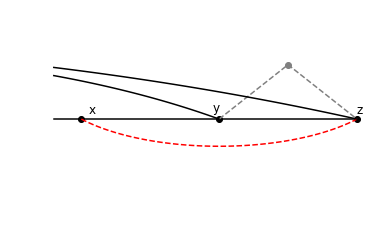
\includegraphics[scale=0.5]{picrel/only_last_reused.png}
  \caption{Только последняя вершина использована повторно. Черным обозначены вершины и рёбра $\tilde H_{k'sm}$, серым вершины и рёбра  $H_{k'sm}$, красным пунктиром~--- рёбра, запрещённые формулой  }
  \label{fig:only last reused}
\end{figure}
\item
она и какая-то до неё: $\tilde \rho^{max} \geq \dfrac{e-2}{v-2}.$ 
\begin{figure}
  \centering
  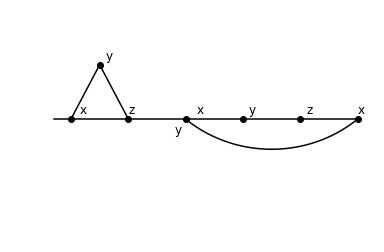
\includegraphics[scale=0.5]{picrel/reuse_intermediate.png}
  \caption{Повторное использование промежуточной вершины}
  \label{fig:reuse intermediate}
\end{figure}
\label{enum:reuse intermediate}
Действительно, посмотрим на первую повторно использованную вершину.
Т.к. формула запрещает совпадать вершинам, соответствующим разным переменным, для её соединения с предыдущими вершинами необходимо добавить ребро, которого нет в графе $H_{k'sm}$. 
С каждой новой секцией в $H_{k'sm}$ добавляется $3+m$ рёбер  и $2+m$ вершин.
Однако, проведя дополнительное ребро к уже имеющейся вершине, мы уже добавили на одно ребро больше, чем вершин, поэтому имеем рёбер $ \tilde e' = e - (3+m) + (\nu+1) = e - (m-\nu) $, вершин $\tilde v' = v - (2+m) + \nu = v - (m-\nu)$, где $\nu$~--- число вершин, уже добавленных в последней ``секции'' $\tilde H_{k'sm}$.
В рассматриваемом случае $\tilde v \leq v-2$, поэтому $\tilde \rho^{max} \geq \frac{e-2}{v-2}$ .
\end{enumerate}
\item
Последняя вершина ещё не была использована:
$\tilde \rho^{max} \geq \dfrac{e}{v-1}.$
Этот случай похож на \ref{enum:reuse intermediate}, но теперь $\tilde v \leq v-1$ и последняя вершина добавляет 2 ребра.
\end{enumerate}

Итого 
$\tilde \rho^{max} \geq \min \left\{\dfrac{e-2}{v-2}, \dfrac{e}{v-1}\right\} = \dfrac{e-2}{v-2} = \dfrac{4+s +(3+m)k'}{3+s + (2+m)k'}$. 

Используя $m=s+2$, получаем $\tilde \rho^{max} - \rho_\infty = \dfrac{1}{((2+m)(k+1)-1)(m+2)}$, следовательно
$\tilde \rho^{max} > \rho_\infty > \rho(H_{ksm}) $.

\end{proof}

Пусть $\alpha = 1/\rho(H_{ksm})$, $m=s+2$.
Пусть  $A$~--- событие, заключающееся в том, что $\Gna$ не содержит подграфов на не более чем $|V(H_{ksm})|$ вершинах с плотностью большей $1/\alpha$.
По лемме \ref{lem:min_ro_Hksm}
\[
A \rightarrow \left[\left(\Gna \vDash \varphi_{ksm} \right) \rightarrow \left(H_{ksm} \subset \Gna \right) \right] .
\]
Выше мы сказали, что, запрещая в формуле $\varphi_{ksm}$ проведение некоторых рёбер между вершинами гантели, мы а.п.н. не теряем того свойства, что формула остаётся истинна всегда, когда $\Gna$ содержит $H_{ksm}$.
Действительно, так как добавление дополнительных рёбер делает $H_{ksm}$ плотнее, чем $1/\alpha$, то получаем
\[
A \rightarrow \left[\left(H_{ksm} \subset \Gna \right) \rightarrow \left(\Gna \vDash \varphi_{ksm} \right)  \right] .
\]
 
По  теореме \ref{th:ruchinski} $\P(A) \rightarrow 1$, поэтому а.п.н. 
\[\left(H_{ksm} \subset \Gna \right) \leftrightarrow \left(\Gna \vDash \varphi_{ksm} \right).\]

Отсюда и из теоремы \ref{th:bollobash} следует

\begin{theorem}
\label{th:my limiting points}
 Закон нуля или единицы для языка $\LL^3$ нарушается в точках $\alpha = \cfrac{m+3 + (2+m)k}{m+4 + (3+m)k}$, $m \geq 3$, $k \geq 0$.
У языка $\LL^3$ есть предельные точки в любой левой полуокрестности единицы.
\end{theorem}